% Options for packages loaded elsewhere
\PassOptionsToPackage{unicode}{hyperref}
\PassOptionsToPackage{hyphens}{url}
%
\documentclass[
]{article}
\usepackage{amsmath,amssymb}
\usepackage{iftex}
\ifPDFTeX
  \usepackage[T1]{fontenc}
  \usepackage[utf8]{inputenc}
  \usepackage{textcomp} % provide euro and other symbols
\else % if luatex or xetex
  \usepackage{unicode-math} % this also loads fontspec
  \defaultfontfeatures{Scale=MatchLowercase}
  \defaultfontfeatures[\rmfamily]{Ligatures=TeX,Scale=1}
\fi
\usepackage{lmodern}
\ifPDFTeX\else
  % xetex/luatex font selection
\fi
% Use upquote if available, for straight quotes in verbatim environments
\IfFileExists{upquote.sty}{\usepackage{upquote}}{}
\IfFileExists{microtype.sty}{% use microtype if available
  \usepackage[]{microtype}
  \UseMicrotypeSet[protrusion]{basicmath} % disable protrusion for tt fonts
}{}
\makeatletter
\@ifundefined{KOMAClassName}{% if non-KOMA class
  \IfFileExists{parskip.sty}{%
    \usepackage{parskip}
  }{% else
    \setlength{\parindent}{0pt}
    \setlength{\parskip}{6pt plus 2pt minus 1pt}}
}{% if KOMA class
  \KOMAoptions{parskip=half}}
\makeatother
\usepackage{xcolor}
\usepackage[margin=1in]{geometry}
\usepackage{color}
\usepackage{fancyvrb}
\newcommand{\VerbBar}{|}
\newcommand{\VERB}{\Verb[commandchars=\\\{\}]}
\DefineVerbatimEnvironment{Highlighting}{Verbatim}{commandchars=\\\{\}}
% Add ',fontsize=\small' for more characters per line
\usepackage{framed}
\definecolor{shadecolor}{RGB}{248,248,248}
\newenvironment{Shaded}{\begin{snugshade}}{\end{snugshade}}
\newcommand{\AlertTok}[1]{\textcolor[rgb]{0.94,0.16,0.16}{#1}}
\newcommand{\AnnotationTok}[1]{\textcolor[rgb]{0.56,0.35,0.01}{\textbf{\textit{#1}}}}
\newcommand{\AttributeTok}[1]{\textcolor[rgb]{0.13,0.29,0.53}{#1}}
\newcommand{\BaseNTok}[1]{\textcolor[rgb]{0.00,0.00,0.81}{#1}}
\newcommand{\BuiltInTok}[1]{#1}
\newcommand{\CharTok}[1]{\textcolor[rgb]{0.31,0.60,0.02}{#1}}
\newcommand{\CommentTok}[1]{\textcolor[rgb]{0.56,0.35,0.01}{\textit{#1}}}
\newcommand{\CommentVarTok}[1]{\textcolor[rgb]{0.56,0.35,0.01}{\textbf{\textit{#1}}}}
\newcommand{\ConstantTok}[1]{\textcolor[rgb]{0.56,0.35,0.01}{#1}}
\newcommand{\ControlFlowTok}[1]{\textcolor[rgb]{0.13,0.29,0.53}{\textbf{#1}}}
\newcommand{\DataTypeTok}[1]{\textcolor[rgb]{0.13,0.29,0.53}{#1}}
\newcommand{\DecValTok}[1]{\textcolor[rgb]{0.00,0.00,0.81}{#1}}
\newcommand{\DocumentationTok}[1]{\textcolor[rgb]{0.56,0.35,0.01}{\textbf{\textit{#1}}}}
\newcommand{\ErrorTok}[1]{\textcolor[rgb]{0.64,0.00,0.00}{\textbf{#1}}}
\newcommand{\ExtensionTok}[1]{#1}
\newcommand{\FloatTok}[1]{\textcolor[rgb]{0.00,0.00,0.81}{#1}}
\newcommand{\FunctionTok}[1]{\textcolor[rgb]{0.13,0.29,0.53}{\textbf{#1}}}
\newcommand{\ImportTok}[1]{#1}
\newcommand{\InformationTok}[1]{\textcolor[rgb]{0.56,0.35,0.01}{\textbf{\textit{#1}}}}
\newcommand{\KeywordTok}[1]{\textcolor[rgb]{0.13,0.29,0.53}{\textbf{#1}}}
\newcommand{\NormalTok}[1]{#1}
\newcommand{\OperatorTok}[1]{\textcolor[rgb]{0.81,0.36,0.00}{\textbf{#1}}}
\newcommand{\OtherTok}[1]{\textcolor[rgb]{0.56,0.35,0.01}{#1}}
\newcommand{\PreprocessorTok}[1]{\textcolor[rgb]{0.56,0.35,0.01}{\textit{#1}}}
\newcommand{\RegionMarkerTok}[1]{#1}
\newcommand{\SpecialCharTok}[1]{\textcolor[rgb]{0.81,0.36,0.00}{\textbf{#1}}}
\newcommand{\SpecialStringTok}[1]{\textcolor[rgb]{0.31,0.60,0.02}{#1}}
\newcommand{\StringTok}[1]{\textcolor[rgb]{0.31,0.60,0.02}{#1}}
\newcommand{\VariableTok}[1]{\textcolor[rgb]{0.00,0.00,0.00}{#1}}
\newcommand{\VerbatimStringTok}[1]{\textcolor[rgb]{0.31,0.60,0.02}{#1}}
\newcommand{\WarningTok}[1]{\textcolor[rgb]{0.56,0.35,0.01}{\textbf{\textit{#1}}}}
\usepackage{longtable,booktabs,array}
\usepackage{calc} % for calculating minipage widths
% Correct order of tables after \paragraph or \subparagraph
\usepackage{etoolbox}
\makeatletter
\patchcmd\longtable{\par}{\if@noskipsec\mbox{}\fi\par}{}{}
\makeatother
% Allow footnotes in longtable head/foot
\IfFileExists{footnotehyper.sty}{\usepackage{footnotehyper}}{\usepackage{footnote}}
\makesavenoteenv{longtable}
\usepackage{graphicx}
\makeatletter
\newsavebox\pandoc@box
\newcommand*\pandocbounded[1]{% scales image to fit in text height/width
  \sbox\pandoc@box{#1}%
  \Gscale@div\@tempa{\textheight}{\dimexpr\ht\pandoc@box+\dp\pandoc@box\relax}%
  \Gscale@div\@tempb{\linewidth}{\wd\pandoc@box}%
  \ifdim\@tempb\p@<\@tempa\p@\let\@tempa\@tempb\fi% select the smaller of both
  \ifdim\@tempa\p@<\p@\scalebox{\@tempa}{\usebox\pandoc@box}%
  \else\usebox{\pandoc@box}%
  \fi%
}
% Set default figure placement to htbp
\def\fps@figure{htbp}
\makeatother
\setlength{\emergencystretch}{3em} % prevent overfull lines
\providecommand{\tightlist}{%
  \setlength{\itemsep}{0pt}\setlength{\parskip}{0pt}}
\setcounter{secnumdepth}{-\maxdimen} % remove section numbering
\usepackage{bookmark}
\IfFileExists{xurl.sty}{\usepackage{xurl}}{} % add URL line breaks if available
\urlstyle{same}
\hypersetup{
  pdftitle={SHC 798 R-code},
  pdfauthor={Richard Lubega},
  hidelinks,
  pdfcreator={LaTeX via pandoc}}

\title{SHC 798 R-code}
\author{Richard Lubega}
\date{2025-07-02}

\begin{document}
\maketitle

\section{Introduction}\label{introduction}

\subsection{R Markdown Preamble}\label{r-markdown-preamble}

This is an R Markdown document. Markdown is a simple formatting syntax
for authoring HTML, PDF, and MS Word documents. For more details on
using R Markdown see \url{http://rmarkdown.rstudio.com}.

When you click the \textbf{Knit} button a document will be generated
that includes both content as well as the output of any embedded R code
chunks within the document. You can embed an R code chunk like this:

\subsection{Sample Inbuilt Data Set}\label{sample-inbuilt-data-set}

\begin{Shaded}
\begin{Highlighting}[]
\FunctionTok{summary}\NormalTok{(cars)}
\end{Highlighting}
\end{Shaded}

\begin{verbatim}
##      speed           dist       
##  Min.   : 4.0   Min.   :  2.00  
##  1st Qu.:12.0   1st Qu.: 26.00  
##  Median :15.0   Median : 36.00  
##  Mean   :15.4   Mean   : 42.98  
##  3rd Qu.:19.0   3rd Qu.: 56.00  
##  Max.   :25.0   Max.   :120.00
\end{verbatim}

\subsection{Including Plots - Example}\label{including-plots---example}

\subsubsection{Embed Plot}\label{embed-plot}

You can also embed plots, for example:

\pandocbounded{\includegraphics[keepaspectratio]{SHC-798-R-code_files/figure-latex/pressure-1.pdf}}

Note that the \texttt{echo\ =\ FALSE} parameter was added to the code
chunk to prevent printing of the R code that generated the plot.

\subsubsection{Another Plot}\label{another-plot}

Let's create another Test plot

\begin{Shaded}
\begin{Highlighting}[]
\FunctionTok{plot}\NormalTok{(cars,  }\AttributeTok{col =} \StringTok{"red"}\NormalTok{, }\AttributeTok{xlab =} \StringTok{"Speed (mph)"}\NormalTok{, }\AttributeTok{ylab =} \StringTok{"Distance (miles)"}\NormalTok{ )}
\end{Highlighting}
\end{Shaded}

\pandocbounded{\includegraphics[keepaspectratio]{SHC-798-R-code_files/figure-latex/test-plot-1.pdf}}

A summary of the data frame is given below

\begin{Shaded}
\begin{Highlighting}[]
\NormalTok{pacman}\SpecialCharTok{::}\FunctionTok{p\_load}\NormalTok{(knitr)}
\FunctionTok{kable}\NormalTok{(}\FunctionTok{summary}\NormalTok{(cars))}
\end{Highlighting}
\end{Shaded}

\begin{longtable}[]{@{}lll@{}}
\toprule\noalign{}
& speed & dist \\
\midrule\noalign{}
\endhead
\bottomrule\noalign{}
\endlastfoot
& Min. : 4.0 & Min. : 2.00 \\
& 1st Qu.:12.0 & 1st Qu.: 26.00 \\
& Median :15.0 & Median : 36.00 \\
& Mean :15.4 & Mean : 42.98 \\
& 3rd Qu.:19.0 & 3rd Qu.: 56.00 \\
& Max. :25.0 & Max. :120.00 \\
\end{longtable}

\section{Start of My SHC 798 R-code}\label{start-of-my-shc-798-r-code}

\subsection{R basics}\label{r-basics}

\begin{enumerate}
\def\labelenumi{\arabic{enumi}.}
\item
  Why install
  \href{https://cran.r-project.org/bin/windows/Rtools/}{\textbf{Rtools}}?
\item
  R Shiny \href{http://shiny.rstudio.com/gallery/}{\textbf{Gallery}}:
  There's Shiny for R and Shiny for Python
\end{enumerate}

\subsection{R Operations 1}\label{r-operations-1}

What can be done?

\begin{Shaded}
\begin{Highlighting}[]
\CommentTok{\# R as a calculator}
\FunctionTok{sqrt}\NormalTok{(}\DecValTok{12}\NormalTok{)}
\end{Highlighting}
\end{Shaded}

\begin{verbatim}
## [1] 3.464102
\end{verbatim}

\begin{Shaded}
\begin{Highlighting}[]
\NormalTok{x }\OtherTok{\textless{}{-}} \DecValTok{3}
\NormalTok{y }\OtherTok{\textless{}{-}}\NormalTok{ x}\SpecialCharTok{\^{}}\DecValTok{2}
\NormalTok{x}\SpecialCharTok{+}\NormalTok{y}
\end{Highlighting}
\end{Shaded}

\begin{verbatim}
## [1] 12
\end{verbatim}

\begin{Shaded}
\begin{Highlighting}[]
\CommentTok{\# Creating Vectors}
\NormalTok{v1 }\OtherTok{\textless{}{-}} \FunctionTok{c}\NormalTok{(}\DecValTok{1}\NormalTok{,}\DecValTok{5}\NormalTok{, }\DecValTok{80}\NormalTok{)}
\NormalTok{v1}
\end{Highlighting}
\end{Shaded}

\begin{verbatim}
## [1]  1  5 80
\end{verbatim}

\begin{Shaded}
\begin{Highlighting}[]
\NormalTok{v2 }\OtherTok{\textless{}{-}} \DecValTok{2}\SpecialCharTok{:}\DecValTok{11}
\NormalTok{v2}
\end{Highlighting}
\end{Shaded}

\begin{verbatim}
##  [1]  2  3  4  5  6  7  8  9 10 11
\end{verbatim}

\begin{Shaded}
\begin{Highlighting}[]
\NormalTok{a }\OtherTok{\textless{}{-}} \FunctionTok{c}\NormalTok{(}\DecValTok{1}\NormalTok{,}\DecValTok{6}\NormalTok{,}\DecValTok{10}\NormalTok{,}\DecValTok{22}\NormalTok{,}\DecValTok{7}\NormalTok{,}\DecValTok{13}\NormalTok{)}
\FunctionTok{mean}\NormalTok{(a)}
\end{Highlighting}
\end{Shaded}

\begin{verbatim}
## [1] 9.833333
\end{verbatim}

\begin{Shaded}
\begin{Highlighting}[]
\CommentTok{\# Incomplete Statement}
\DecValTok{3}\SpecialCharTok{*}\NormalTok{(}\DecValTok{4} \SpecialCharTok{+}
     \SpecialCharTok{+}\DecValTok{2}\NormalTok{)}
\end{Highlighting}
\end{Shaded}

\begin{verbatim}
## [1] 18
\end{verbatim}

\begin{Shaded}
\begin{Highlighting}[]
\CommentTok{\#Assignments and Function Calls}
\NormalTok{t.a }\OtherTok{\textless{}{-}} \DecValTok{3}\SpecialCharTok{*}\NormalTok{(}\DecValTok{4}\SpecialCharTok{+}\DecValTok{2}\NormalTok{)}
\NormalTok{t.b }\OtherTok{\textless{}{-}}\NormalTok{ t.a }\SpecialCharTok{+} \FloatTok{2.5}
\NormalTok{mn }\OtherTok{\textless{}{-}} \FunctionTok{mean}\NormalTok{(}\FunctionTok{c}\NormalTok{(t.a,t.b))}
\NormalTok{mn}
\end{Highlighting}
\end{Shaded}

\begin{verbatim}
## [1] 19.25
\end{verbatim}

\subsection{R Help}\label{r-help}

Resources

\begin{enumerate}
\def\labelenumi{\arabic{enumi}.}
\item
  Very useful and helpful \href{http://stackexchange.com/}{\textbf{R
  Q\&A Website}}
\item
  Paradis 2005 - R for Beginners {[}Textbook{]}
\item
  R Reference Card {[}in the notes, 6 pages - Material from \emph{R for
  Beginners}{]}
\item
  Base R Cheat Sheet {[}in the notes, 2 pages{]}
\item
  Venables et al 2017 - An introduction to R {[}Textbook{]}
\item
  \href{https://r4ds.had.co.nz/index.html}{\textbf{R for Data Science,
  r4ds}} or the \href{https://r4ds.hadley.nz/}{\textbf{r4ds-2e}}
\item
  \href{https://www.w3schools.com/r/default.asp}{\textbf{W\textsuperscript{3}Schools}}
  R Certification
\end{enumerate}

\begin{figure}
\centering
\pandocbounded{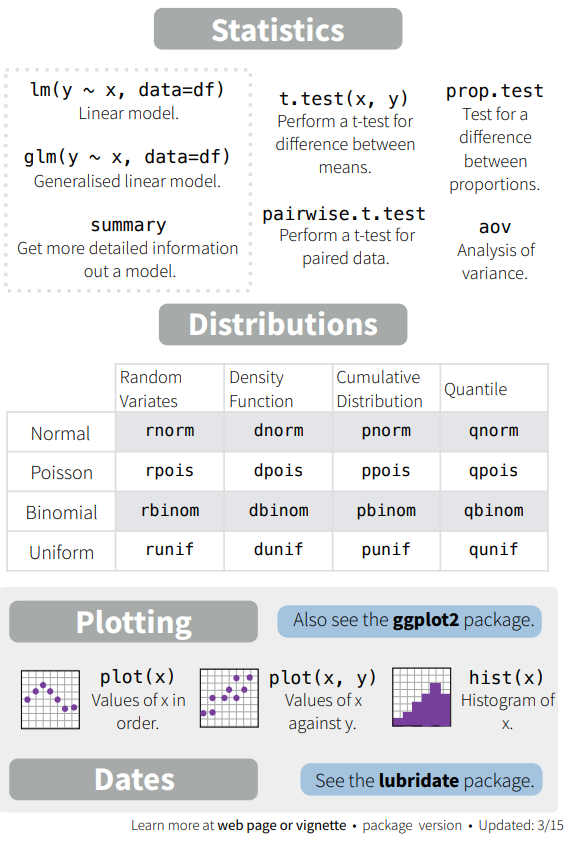
\includegraphics[keepaspectratio]{R-Statistics.png}}
\caption{\emph{Snippet from Resource 4}}
\end{figure}

\subsection{R Operations 2}\label{r-operations-2}

\subsubsection{Importing Data sets}\label{importing-data-sets}

\begin{Shaded}
\begin{Highlighting}[]
\CommentTok{\# Import Data: Website}
\NormalTok{url }\OtherTok{\textless{}{-}} \StringTok{"https://stat.ethz.ch/Teaching/Datasets/WBL/sport.dat"}
\NormalTok{d.sport }\OtherTok{\textless{}{-}} \FunctionTok{read.table}\NormalTok{(url, }\AttributeTok{header =} \ConstantTok{TRUE}\NormalTok{)}
\FunctionTok{head}\NormalTok{(d.sport)}
\end{Highlighting}
\end{Shaded}

\begin{verbatim}
##            weit kugel hoch  disc stab speer punkte
## OBRIEN     7.57 15.66  207 48.78  500 66.90   8824
## BUSEMANN   8.07 13.60  204 45.04  480 66.86   8706
## DVORAK     7.60 15.82  198 46.28  470 70.16   8664
## FRITZ      7.77 15.31  204 49.84  510 65.70   8644
## HAMALAINEN 7.48 16.32  198 49.62  500 57.66   8613
## NOOL       7.88 14.01  201 42.98  540 65.48   8543
\end{verbatim}

\begin{Shaded}
\begin{Highlighting}[]
\CommentTok{\# Setting the Working Directory}
\CommentTok{\# Use:}
\FunctionTok{getwd}\NormalTok{() }\CommentTok{\#Prints the current working directory}
\end{Highlighting}
\end{Shaded}

\begin{verbatim}
## [1] "D:/2025 MEng Transportation/SHC 798 R-Proj"
\end{verbatim}

\begin{Shaded}
\begin{Highlighting}[]
\CommentTok{\# setwd("D:/2025 MEng Transportation/SHC 798 R{-}Proj") \textasciitilde{} Sets the working directory}
\CommentTok{\# Alternatively, use “Session” → “Set Working Directory” → “Choose Directory…”}
\CommentTok{\# Import Data: Files}
  \CommentTok{\# {-} Different ways depending on the format (csv, txt, xlsx, etc.) }
  \CommentTok{\# {-} Alternative: use the “Import Dataset” tool in RStudio (upper{-}right panel)}
\CommentTok{\# Save data or write data to a file}
  \CommentTok{\# {-} Text files}
  \CommentTok{\# {-} Excel files: use CSV}
\end{Highlighting}
\end{Shaded}

\subsubsection{R Objects \& Indexing}\label{r-objects-indexing}

\begin{Shaded}
\begin{Highlighting}[]
\CommentTok{\# R Objects: Data frames (Most essential)}
\FunctionTok{str}\NormalTok{(d.sport)}
\end{Highlighting}
\end{Shaded}

\begin{verbatim}
## 'data.frame':    15 obs. of  7 variables:
##  $ weit  : num  7.57 8.07 7.6 7.77 7.48 7.88 7.64 7.61 7.27 7.49 ...
##  $ kugel : num  15.7 13.6 15.8 15.3 16.3 ...
##  $ hoch  : int  207 204 198 204 198 201 195 213 207 204 ...
##  $ disc  : num  48.8 45 46.3 49.8 49.6 ...
##  $ stab  : int  500 480 470 510 500 540 540 520 470 470 ...
##  $ speer : num  66.9 66.9 70.2 65.7 57.7 ...
##  $ punkte: int  8824 8706 8664 8644 8613 8543 8422 8318 8307 8300 ...
\end{verbatim}

\begin{Shaded}
\begin{Highlighting}[]
\CommentTok{\# R Objects: Vectors}
  \CommentTok{\# (e.g., a column from the data set d.sport)}
\NormalTok{kugel }\OtherTok{\textless{}{-}}\NormalTok{ d.sport}\SpecialCharTok{$}\NormalTok{kugel}
\FunctionTok{str}\NormalTok{(kugel)}
\end{Highlighting}
\end{Shaded}

\begin{verbatim}
##  num [1:15] 15.7 13.6 15.8 15.3 16.3 ...
\end{verbatim}

\begin{Shaded}
\begin{Highlighting}[]
\NormalTok{participant }\OtherTok{\textless{}{-}} \FunctionTok{rownames}\NormalTok{(d.sport)}
\FunctionTok{str}\NormalTok{(participant)}
\end{Highlighting}
\end{Shaded}

\begin{verbatim}
##  chr [1:15] "OBRIEN" "BUSEMANN" "DVORAK" "FRITZ" "HAMALAINEN" "NOOL" ...
\end{verbatim}

\begin{Shaded}
\begin{Highlighting}[]
\CommentTok{\# Select elements}
\NormalTok{participant[}\DecValTok{4}\NormalTok{]}
\end{Highlighting}
\end{Shaded}

\begin{verbatim}
## [1] "FRITZ"
\end{verbatim}

\begin{Shaded}
\begin{Highlighting}[]
\NormalTok{d.sport[}\FunctionTok{c}\NormalTok{(}\DecValTok{3}\NormalTok{,}\DecValTok{6}\NormalTok{,}\DecValTok{4}\NormalTok{), }\FunctionTok{c}\NormalTok{(}\DecValTok{1}\SpecialCharTok{:}\DecValTok{3}\NormalTok{,}\DecValTok{7}\NormalTok{)]}
\end{Highlighting}
\end{Shaded}

\begin{verbatim}
##        weit kugel hoch punkte
## DVORAK 7.60 15.82  198   8664
## NOOL   7.88 14.01  201   8543
## FRITZ  7.77 15.31  204   8644
\end{verbatim}

\begin{Shaded}
\begin{Highlighting}[]
\NormalTok{d.sport[}\StringTok{"FRITZ"}\NormalTok{, ]}
\end{Highlighting}
\end{Shaded}

\begin{verbatim}
##       weit kugel hoch  disc stab speer punkte
## FRITZ 7.77 15.31  204 49.84  510  65.7   8644
\end{verbatim}

\begin{Shaded}
\begin{Highlighting}[]
\CommentTok{\# Accessing Parts of an Object}
\CommentTok{\# To access only part of an object, use []}
  \CommentTok{\# For vectors: myvector[x]}
  \CommentTok{\# For two{-}dimensional objects, e.g. data frames or matrices: mydata.frame[x,y]}
\NormalTok{d.sport[ , ]}
\end{Highlighting}
\end{Shaded}

\begin{verbatim}
##            weit kugel hoch  disc stab speer punkte
## OBRIEN     7.57 15.66  207 48.78  500 66.90   8824
## BUSEMANN   8.07 13.60  204 45.04  480 66.86   8706
## DVORAK     7.60 15.82  198 46.28  470 70.16   8664
## FRITZ      7.77 15.31  204 49.84  510 65.70   8644
## HAMALAINEN 7.48 16.32  198 49.62  500 57.66   8613
## NOOL       7.88 14.01  201 42.98  540 65.48   8543
## ZMELIK     7.64 13.53  195 43.44  540 67.20   8422
## GANIYEV    7.61 14.71  213 44.86  520 53.70   8318
## PENALVER   7.27 16.91  207 48.92  470 57.08   8307
## HUFFINS    7.49 15.57  204 48.72  470 60.62   8300
## PLAZIAT    7.82 14.85  204 45.34  490 52.18   8282
## MAGNUSSON  7.28 15.52  195 43.78  480 61.10   8274
## SMITH      7.47 16.97  195 49.54  500 64.34   8271
## MUELLER    7.25 14.69  195 45.90  510 66.10   8253
## CHMARA     7.75 14.51  210 42.60  490 54.84   8249
\end{verbatim}

\begin{Shaded}
\begin{Highlighting}[]
\FunctionTok{c}\NormalTok{(}\DecValTok{1}\NormalTok{,}\DecValTok{3}\NormalTok{,}\DecValTok{7}\NormalTok{)}
\end{Highlighting}
\end{Shaded}

\begin{verbatim}
## [1] 1 3 7
\end{verbatim}

\begin{Shaded}
\begin{Highlighting}[]
\DecValTok{1}\SpecialCharTok{:}\DecValTok{10}
\end{Highlighting}
\end{Shaded}

\begin{verbatim}
##  [1]  1  2  3  4  5  6  7  8  9 10
\end{verbatim}

\begin{Shaded}
\begin{Highlighting}[]
\NormalTok{d.sport[}\DecValTok{1}\SpecialCharTok{:}\DecValTok{10}\NormalTok{, ]}
\end{Highlighting}
\end{Shaded}

\begin{verbatim}
##            weit kugel hoch  disc stab speer punkte
## OBRIEN     7.57 15.66  207 48.78  500 66.90   8824
## BUSEMANN   8.07 13.60  204 45.04  480 66.86   8706
## DVORAK     7.60 15.82  198 46.28  470 70.16   8664
## FRITZ      7.77 15.31  204 49.84  510 65.70   8644
## HAMALAINEN 7.48 16.32  198 49.62  500 57.66   8613
## NOOL       7.88 14.01  201 42.98  540 65.48   8543
## ZMELIK     7.64 13.53  195 43.44  540 67.20   8422
## GANIYEV    7.61 14.71  213 44.86  520 53.70   8318
## PENALVER   7.27 16.91  207 48.92  470 57.08   8307
## HUFFINS    7.49 15.57  204 48.72  470 60.62   8300
\end{verbatim}

\begin{Shaded}
\begin{Highlighting}[]
\NormalTok{d.sport[}\SpecialCharTok{{-}}\FunctionTok{c}\NormalTok{(}\DecValTok{1}\NormalTok{, }\DecValTok{3}\NormalTok{,}\DecValTok{7}\NormalTok{), ] }\CommentTok{\#negative indices are excluded}
\end{Highlighting}
\end{Shaded}

\begin{verbatim}
##            weit kugel hoch  disc stab speer punkte
## BUSEMANN   8.07 13.60  204 45.04  480 66.86   8706
## FRITZ      7.77 15.31  204 49.84  510 65.70   8644
## HAMALAINEN 7.48 16.32  198 49.62  500 57.66   8613
## NOOL       7.88 14.01  201 42.98  540 65.48   8543
## GANIYEV    7.61 14.71  213 44.86  520 53.70   8318
## PENALVER   7.27 16.91  207 48.92  470 57.08   8307
## HUFFINS    7.49 15.57  204 48.72  470 60.62   8300
## PLAZIAT    7.82 14.85  204 45.34  490 52.18   8282
## MAGNUSSON  7.28 15.52  195 43.78  480 61.10   8274
## SMITH      7.47 16.97  195 49.54  500 64.34   8271
## MUELLER    7.25 14.69  195 45.90  510 66.10   8253
## CHMARA     7.75 14.51  210 42.60  490 54.84   8249
\end{verbatim}

\begin{Shaded}
\begin{Highlighting}[]
\NormalTok{d.sport[ , }\DecValTok{2}\SpecialCharTok{:}\DecValTok{3}\NormalTok{]}
\end{Highlighting}
\end{Shaded}

\begin{verbatim}
##            kugel hoch
## OBRIEN     15.66  207
## BUSEMANN   13.60  204
## DVORAK     15.82  198
## FRITZ      15.31  204
## HAMALAINEN 16.32  198
## NOOL       14.01  201
## ZMELIK     13.53  195
## GANIYEV    14.71  213
## PENALVER   16.91  207
## HUFFINS    15.57  204
## PLAZIAT    14.85  204
## MAGNUSSON  15.52  195
## SMITH      16.97  195
## MUELLER    14.69  195
## CHMARA     14.51  210
\end{verbatim}

\begin{Shaded}
\begin{Highlighting}[]
\NormalTok{d.sport[}\FunctionTok{c}\NormalTok{(}\DecValTok{1}\NormalTok{,}\DecValTok{3}\NormalTok{,}\DecValTok{6}\NormalTok{), }\DecValTok{2}\SpecialCharTok{:}\DecValTok{3}\NormalTok{]}
\end{Highlighting}
\end{Shaded}

\begin{verbatim}
##        kugel hoch
## OBRIEN 15.66  207
## DVORAK 15.82  198
## NOOL   14.01  201
\end{verbatim}

\begin{Shaded}
\begin{Highlighting}[]
\CommentTok{\# Function Calls}
\FunctionTok{mean}\NormalTok{(kugel)}
\end{Highlighting}
\end{Shaded}

\begin{verbatim}
## [1] 15.19867
\end{verbatim}

\begin{Shaded}
\begin{Highlighting}[]
\FunctionTok{quantile}\NormalTok{(kugel)}
\end{Highlighting}
\end{Shaded}

\begin{verbatim}
##    0%   25%   50%   75%  100% 
## 13.53 14.60 15.31 15.74 16.97
\end{verbatim}

\begin{Shaded}
\begin{Highlighting}[]
\FunctionTok{quantile}\NormalTok{(kugel,}\AttributeTok{probs =} \FunctionTok{c}\NormalTok{(.}\DecValTok{75}\NormalTok{, }\FloatTok{0.9}\NormalTok{))}
\end{Highlighting}
\end{Shaded}

\begin{verbatim}
##    75%    90% 
## 15.740 16.674
\end{verbatim}

\begin{Shaded}
\begin{Highlighting}[]
\CommentTok{\# Functions consist of mandatory and optional arguments:}
  \CommentTok{\# mean(x, trim = 0, na.rm = FALSE, …)}
  \CommentTok{\# x: mandatory argument}
  \CommentTok{\# trim: optional argument, default is 0}
  \CommentTok{\# na.rm: optional argument, default is FALSE}

\CommentTok{\# The arguments of a function have a defined order and each argument has its own unique name}
\FunctionTok{mean}\NormalTok{(}\AttributeTok{x =}\NormalTok{ kugel, }\AttributeTok{na.rm =} \ConstantTok{TRUE}\NormalTok{)}
\end{Highlighting}
\end{Shaded}

\begin{verbatim}
## [1] 15.19867
\end{verbatim}

\begin{Shaded}
\begin{Highlighting}[]
\FunctionTok{mean}\NormalTok{(}\AttributeTok{x =}\NormalTok{ kugel, ,}\ConstantTok{TRUE}\NormalTok{)}
\end{Highlighting}
\end{Shaded}

\begin{verbatim}
## [1] 15.19867
\end{verbatim}

\begin{Shaded}
\begin{Highlighting}[]
\CommentTok{\# Useful Functions}
\FunctionTok{nrow}\NormalTok{(d.sport)}
\end{Highlighting}
\end{Shaded}

\begin{verbatim}
## [1] 15
\end{verbatim}

\begin{Shaded}
\begin{Highlighting}[]
\FunctionTok{ncol}\NormalTok{(d.sport)}
\end{Highlighting}
\end{Shaded}

\begin{verbatim}
## [1] 7
\end{verbatim}

\begin{Shaded}
\begin{Highlighting}[]
\FunctionTok{dim}\NormalTok{(d.sport)}
\end{Highlighting}
\end{Shaded}

\begin{verbatim}
## [1] 15  7
\end{verbatim}

\begin{Shaded}
\begin{Highlighting}[]
\FunctionTok{summary}\NormalTok{(d.sport)}
\end{Highlighting}
\end{Shaded}

\begin{verbatim}
##       weit           kugel            hoch            disc            stab    
##  Min.   :7.250   Min.   :13.53   Min.   :195.0   Min.   :42.60   Min.   :470  
##  1st Qu.:7.475   1st Qu.:14.60   1st Qu.:196.5   1st Qu.:44.32   1st Qu.:480  
##  Median :7.600   Median :15.31   Median :204.0   Median :45.90   Median :500  
##  Mean   :7.597   Mean   :15.20   Mean   :202.0   Mean   :46.38   Mean   :498  
##  3rd Qu.:7.760   3rd Qu.:15.74   3rd Qu.:205.5   3rd Qu.:48.85   3rd Qu.:510  
##  Max.   :8.070   Max.   :16.97   Max.   :213.0   Max.   :49.84   Max.   :540  
##      speer           punkte    
##  Min.   :52.18   Min.   :8249  
##  1st Qu.:57.37   1st Qu.:8278  
##  Median :64.34   Median :8318  
##  Mean   :61.99   Mean   :8445  
##  3rd Qu.:66.48   3rd Qu.:8628  
##  Max.   :70.16   Max.   :8824
\end{verbatim}

\begin{Shaded}
\begin{Highlighting}[]
\CommentTok{\# apply(d.sport)}
\FunctionTok{head}\NormalTok{(d.sport)}
\end{Highlighting}
\end{Shaded}

\begin{verbatim}
##            weit kugel hoch  disc stab speer punkte
## OBRIEN     7.57 15.66  207 48.78  500 66.90   8824
## BUSEMANN   8.07 13.60  204 45.04  480 66.86   8706
## DVORAK     7.60 15.82  198 46.28  470 70.16   8664
## FRITZ      7.77 15.31  204 49.84  510 65.70   8644
## HAMALAINEN 7.48 16.32  198 49.62  500 57.66   8613
## NOOL       7.88 14.01  201 42.98  540 65.48   8543
\end{verbatim}

\begin{Shaded}
\begin{Highlighting}[]
\FunctionTok{tail}\NormalTok{(d.sport)}
\end{Highlighting}
\end{Shaded}

\begin{verbatim}
##           weit kugel hoch  disc stab speer punkte
## HUFFINS   7.49 15.57  204 48.72  470 60.62   8300
## PLAZIAT   7.82 14.85  204 45.34  490 52.18   8282
## MAGNUSSON 7.28 15.52  195 43.78  480 61.10   8274
## SMITH     7.47 16.97  195 49.54  500 64.34   8271
## MUELLER   7.25 14.69  195 45.90  510 66.10   8253
## CHMARA    7.75 14.51  210 42.60  490 54.84   8249
\end{verbatim}

\subsubsection{R Packages}\label{r-packages}

\begin{Shaded}
\begin{Highlighting}[]
\CommentTok{\#install.packages("MASS")}
\CommentTok{\#require(MASS) \# for every R Session}
\CommentTok{\#library(MASS) \# or use this}
\end{Highlighting}
\end{Shaded}

Online resources: University of Pretoria \textbar{} SHC 798 \textbar{}
Introduction to R 36

o List of all packages: \url{http://cran.r-project.org/web/packages/}

o By topic: \url{http://cran.r-project.org/web/views/}

o Ask Google / ChatGPT / GroK

\subsubsection{Missing Values}\label{missing-values}

\begin{Shaded}
\begin{Highlighting}[]
\NormalTok{d.sport.NA }\OtherTok{\textless{}{-}}\NormalTok{ d.sport}
\NormalTok{d.sport.NA[}\DecValTok{2}\NormalTok{, }\StringTok{"kugel"}\NormalTok{] }\OtherTok{\textless{}{-}} \ConstantTok{NA} 
\NormalTok{d.sport.NA[}\DecValTok{3}\NormalTok{, }\StringTok{"hoch"}\NormalTok{] }\OtherTok{\textless{}{-}} \SpecialCharTok{{-}}\DecValTok{999}
\CommentTok{\# missing values are coded as NA (not available) and are treated in a special way, e.g. is.na():}
\FunctionTok{is.na}\NormalTok{(d.sport.NA) }\CommentTok{\#one logical value per element}
\end{Highlighting}
\end{Shaded}

\begin{verbatim}
##             weit kugel  hoch  disc  stab speer punkte
## OBRIEN     FALSE FALSE FALSE FALSE FALSE FALSE  FALSE
## BUSEMANN   FALSE  TRUE FALSE FALSE FALSE FALSE  FALSE
## DVORAK     FALSE FALSE FALSE FALSE FALSE FALSE  FALSE
## FRITZ      FALSE FALSE FALSE FALSE FALSE FALSE  FALSE
## HAMALAINEN FALSE FALSE FALSE FALSE FALSE FALSE  FALSE
## NOOL       FALSE FALSE FALSE FALSE FALSE FALSE  FALSE
## ZMELIK     FALSE FALSE FALSE FALSE FALSE FALSE  FALSE
## GANIYEV    FALSE FALSE FALSE FALSE FALSE FALSE  FALSE
## PENALVER   FALSE FALSE FALSE FALSE FALSE FALSE  FALSE
## HUFFINS    FALSE FALSE FALSE FALSE FALSE FALSE  FALSE
## PLAZIAT    FALSE FALSE FALSE FALSE FALSE FALSE  FALSE
## MAGNUSSON  FALSE FALSE FALSE FALSE FALSE FALSE  FALSE
## SMITH      FALSE FALSE FALSE FALSE FALSE FALSE  FALSE
## MUELLER    FALSE FALSE FALSE FALSE FALSE FALSE  FALSE
## CHMARA     FALSE FALSE FALSE FALSE FALSE FALSE  FALSE
\end{verbatim}

\begin{Shaded}
\begin{Highlighting}[]
\FunctionTok{sum}\NormalTok{(}\FunctionTok{is.na}\NormalTok{(d.sport.NA)) }\CommentTok{\# adds up the TRUE elements}
\end{Highlighting}
\end{Shaded}

\begin{verbatim}
## [1] 1
\end{verbatim}

\begin{Shaded}
\begin{Highlighting}[]
\FunctionTok{which}\NormalTok{(}\FunctionTok{is.na}\NormalTok{(d.sport.NA), }\AttributeTok{arr.ind =} \ConstantTok{TRUE}\NormalTok{) }\CommentTok{\# where are the NA\textquotesingle{}s}
\end{Highlighting}
\end{Shaded}

\begin{verbatim}
##          row col
## BUSEMANN   2   2
\end{verbatim}

\begin{Shaded}
\begin{Highlighting}[]
\CommentTok{\# Specify missing values after reading in the data:}
\NormalTok{d.sport.NA[d.sport.NA }\SpecialCharTok{==} \SpecialCharTok{{-}}\DecValTok{999}\NormalTok{] }\OtherTok{\textless{}{-}} \ConstantTok{NA}

\CommentTok{\# Many functions have an argument to handle missing values, e.g. na.rm, na.omit:}
\FunctionTok{sum}\NormalTok{(d.sport.NA}\SpecialCharTok{$}\NormalTok{kugel)}
\end{Highlighting}
\end{Shaded}

\begin{verbatim}
## [1] NA
\end{verbatim}

\begin{Shaded}
\begin{Highlighting}[]
\FunctionTok{sum}\NormalTok{(d.sport.NA}\SpecialCharTok{$}\NormalTok{kugel, }\AttributeTok{na.rm =} \ConstantTok{TRUE}\NormalTok{)}
\end{Highlighting}
\end{Shaded}

\begin{verbatim}
## [1] 214.38
\end{verbatim}

\begin{Shaded}
\begin{Highlighting}[]
\FunctionTok{na.omit}\NormalTok{(d.sport.NA)}
\end{Highlighting}
\end{Shaded}

\begin{verbatim}
##            weit kugel hoch  disc stab speer punkte
## OBRIEN     7.57 15.66  207 48.78  500 66.90   8824
## FRITZ      7.77 15.31  204 49.84  510 65.70   8644
## HAMALAINEN 7.48 16.32  198 49.62  500 57.66   8613
## NOOL       7.88 14.01  201 42.98  540 65.48   8543
## ZMELIK     7.64 13.53  195 43.44  540 67.20   8422
## GANIYEV    7.61 14.71  213 44.86  520 53.70   8318
## PENALVER   7.27 16.91  207 48.92  470 57.08   8307
## HUFFINS    7.49 15.57  204 48.72  470 60.62   8300
## PLAZIAT    7.82 14.85  204 45.34  490 52.18   8282
## MAGNUSSON  7.28 15.52  195 43.78  480 61.10   8274
## SMITH      7.47 16.97  195 49.54  500 64.34   8271
## MUELLER    7.25 14.69  195 45.90  510 66.10   8253
## CHMARA     7.75 14.51  210 42.60  490 54.84   8249
\end{verbatim}

\subsection{Basic Graphics}\label{basic-graphics}

\begin{Shaded}
\begin{Highlighting}[]
\CommentTok{\# The Plot Function: only 1 mandatory argument i.e., x. The 2nd most important one is y. }
  \CommentTok{\# many optional arguments [col,pch,main,cex, ...]}
  \CommentTok{\# use function par (?par) to set or query graphical parameters}

\FunctionTok{data}\NormalTok{(iris)}
\NormalTok{iris}
\end{Highlighting}
\end{Shaded}

\begin{verbatim}
##     Sepal.Length Sepal.Width Petal.Length Petal.Width    Species
## 1            5.1         3.5          1.4         0.2     setosa
## 2            4.9         3.0          1.4         0.2     setosa
## 3            4.7         3.2          1.3         0.2     setosa
## 4            4.6         3.1          1.5         0.2     setosa
## 5            5.0         3.6          1.4         0.2     setosa
## 6            5.4         3.9          1.7         0.4     setosa
## 7            4.6         3.4          1.4         0.3     setosa
## 8            5.0         3.4          1.5         0.2     setosa
## 9            4.4         2.9          1.4         0.2     setosa
## 10           4.9         3.1          1.5         0.1     setosa
## 11           5.4         3.7          1.5         0.2     setosa
## 12           4.8         3.4          1.6         0.2     setosa
## 13           4.8         3.0          1.4         0.1     setosa
## 14           4.3         3.0          1.1         0.1     setosa
## 15           5.8         4.0          1.2         0.2     setosa
## 16           5.7         4.4          1.5         0.4     setosa
## 17           5.4         3.9          1.3         0.4     setosa
## 18           5.1         3.5          1.4         0.3     setosa
## 19           5.7         3.8          1.7         0.3     setosa
## 20           5.1         3.8          1.5         0.3     setosa
## 21           5.4         3.4          1.7         0.2     setosa
## 22           5.1         3.7          1.5         0.4     setosa
## 23           4.6         3.6          1.0         0.2     setosa
## 24           5.1         3.3          1.7         0.5     setosa
## 25           4.8         3.4          1.9         0.2     setosa
## 26           5.0         3.0          1.6         0.2     setosa
## 27           5.0         3.4          1.6         0.4     setosa
## 28           5.2         3.5          1.5         0.2     setosa
## 29           5.2         3.4          1.4         0.2     setosa
## 30           4.7         3.2          1.6         0.2     setosa
## 31           4.8         3.1          1.6         0.2     setosa
## 32           5.4         3.4          1.5         0.4     setosa
## 33           5.2         4.1          1.5         0.1     setosa
## 34           5.5         4.2          1.4         0.2     setosa
## 35           4.9         3.1          1.5         0.2     setosa
## 36           5.0         3.2          1.2         0.2     setosa
## 37           5.5         3.5          1.3         0.2     setosa
## 38           4.9         3.6          1.4         0.1     setosa
## 39           4.4         3.0          1.3         0.2     setosa
## 40           5.1         3.4          1.5         0.2     setosa
## 41           5.0         3.5          1.3         0.3     setosa
## 42           4.5         2.3          1.3         0.3     setosa
## 43           4.4         3.2          1.3         0.2     setosa
## 44           5.0         3.5          1.6         0.6     setosa
## 45           5.1         3.8          1.9         0.4     setosa
## 46           4.8         3.0          1.4         0.3     setosa
## 47           5.1         3.8          1.6         0.2     setosa
## 48           4.6         3.2          1.4         0.2     setosa
## 49           5.3         3.7          1.5         0.2     setosa
## 50           5.0         3.3          1.4         0.2     setosa
## 51           7.0         3.2          4.7         1.4 versicolor
## 52           6.4         3.2          4.5         1.5 versicolor
## 53           6.9         3.1          4.9         1.5 versicolor
## 54           5.5         2.3          4.0         1.3 versicolor
## 55           6.5         2.8          4.6         1.5 versicolor
## 56           5.7         2.8          4.5         1.3 versicolor
## 57           6.3         3.3          4.7         1.6 versicolor
## 58           4.9         2.4          3.3         1.0 versicolor
## 59           6.6         2.9          4.6         1.3 versicolor
## 60           5.2         2.7          3.9         1.4 versicolor
## 61           5.0         2.0          3.5         1.0 versicolor
## 62           5.9         3.0          4.2         1.5 versicolor
## 63           6.0         2.2          4.0         1.0 versicolor
## 64           6.1         2.9          4.7         1.4 versicolor
## 65           5.6         2.9          3.6         1.3 versicolor
## 66           6.7         3.1          4.4         1.4 versicolor
## 67           5.6         3.0          4.5         1.5 versicolor
## 68           5.8         2.7          4.1         1.0 versicolor
## 69           6.2         2.2          4.5         1.5 versicolor
## 70           5.6         2.5          3.9         1.1 versicolor
## 71           5.9         3.2          4.8         1.8 versicolor
## 72           6.1         2.8          4.0         1.3 versicolor
## 73           6.3         2.5          4.9         1.5 versicolor
## 74           6.1         2.8          4.7         1.2 versicolor
## 75           6.4         2.9          4.3         1.3 versicolor
## 76           6.6         3.0          4.4         1.4 versicolor
## 77           6.8         2.8          4.8         1.4 versicolor
## 78           6.7         3.0          5.0         1.7 versicolor
## 79           6.0         2.9          4.5         1.5 versicolor
## 80           5.7         2.6          3.5         1.0 versicolor
## 81           5.5         2.4          3.8         1.1 versicolor
## 82           5.5         2.4          3.7         1.0 versicolor
## 83           5.8         2.7          3.9         1.2 versicolor
## 84           6.0         2.7          5.1         1.6 versicolor
## 85           5.4         3.0          4.5         1.5 versicolor
## 86           6.0         3.4          4.5         1.6 versicolor
## 87           6.7         3.1          4.7         1.5 versicolor
## 88           6.3         2.3          4.4         1.3 versicolor
## 89           5.6         3.0          4.1         1.3 versicolor
## 90           5.5         2.5          4.0         1.3 versicolor
## 91           5.5         2.6          4.4         1.2 versicolor
## 92           6.1         3.0          4.6         1.4 versicolor
## 93           5.8         2.6          4.0         1.2 versicolor
## 94           5.0         2.3          3.3         1.0 versicolor
## 95           5.6         2.7          4.2         1.3 versicolor
## 96           5.7         3.0          4.2         1.2 versicolor
## 97           5.7         2.9          4.2         1.3 versicolor
## 98           6.2         2.9          4.3         1.3 versicolor
## 99           5.1         2.5          3.0         1.1 versicolor
## 100          5.7         2.8          4.1         1.3 versicolor
## 101          6.3         3.3          6.0         2.5  virginica
## 102          5.8         2.7          5.1         1.9  virginica
## 103          7.1         3.0          5.9         2.1  virginica
## 104          6.3         2.9          5.6         1.8  virginica
## 105          6.5         3.0          5.8         2.2  virginica
## 106          7.6         3.0          6.6         2.1  virginica
## 107          4.9         2.5          4.5         1.7  virginica
## 108          7.3         2.9          6.3         1.8  virginica
## 109          6.7         2.5          5.8         1.8  virginica
## 110          7.2         3.6          6.1         2.5  virginica
## 111          6.5         3.2          5.1         2.0  virginica
## 112          6.4         2.7          5.3         1.9  virginica
## 113          6.8         3.0          5.5         2.1  virginica
## 114          5.7         2.5          5.0         2.0  virginica
## 115          5.8         2.8          5.1         2.4  virginica
## 116          6.4         3.2          5.3         2.3  virginica
## 117          6.5         3.0          5.5         1.8  virginica
## 118          7.7         3.8          6.7         2.2  virginica
## 119          7.7         2.6          6.9         2.3  virginica
## 120          6.0         2.2          5.0         1.5  virginica
## 121          6.9         3.2          5.7         2.3  virginica
## 122          5.6         2.8          4.9         2.0  virginica
## 123          7.7         2.8          6.7         2.0  virginica
## 124          6.3         2.7          4.9         1.8  virginica
## 125          6.7         3.3          5.7         2.1  virginica
## 126          7.2         3.2          6.0         1.8  virginica
## 127          6.2         2.8          4.8         1.8  virginica
## 128          6.1         3.0          4.9         1.8  virginica
## 129          6.4         2.8          5.6         2.1  virginica
## 130          7.2         3.0          5.8         1.6  virginica
## 131          7.4         2.8          6.1         1.9  virginica
## 132          7.9         3.8          6.4         2.0  virginica
## 133          6.4         2.8          5.6         2.2  virginica
## 134          6.3         2.8          5.1         1.5  virginica
## 135          6.1         2.6          5.6         1.4  virginica
## 136          7.7         3.0          6.1         2.3  virginica
## 137          6.3         3.4          5.6         2.4  virginica
## 138          6.4         3.1          5.5         1.8  virginica
## 139          6.0         3.0          4.8         1.8  virginica
## 140          6.9         3.1          5.4         2.1  virginica
## 141          6.7         3.1          5.6         2.4  virginica
## 142          6.9         3.1          5.1         2.3  virginica
## 143          5.8         2.7          5.1         1.9  virginica
## 144          6.8         3.2          5.9         2.3  virginica
## 145          6.7         3.3          5.7         2.5  virginica
## 146          6.7         3.0          5.2         2.3  virginica
## 147          6.3         2.5          5.0         1.9  virginica
## 148          6.5         3.0          5.2         2.0  virginica
## 149          6.2         3.4          5.4         2.3  virginica
## 150          5.9         3.0          5.1         1.8  virginica
\end{verbatim}

\begin{Shaded}
\begin{Highlighting}[]
\FunctionTok{str}\NormalTok{(iris)}
\end{Highlighting}
\end{Shaded}

\begin{verbatim}
## 'data.frame':    150 obs. of  5 variables:
##  $ Sepal.Length: num  5.1 4.9 4.7 4.6 5 5.4 4.6 5 4.4 4.9 ...
##  $ Sepal.Width : num  3.5 3 3.2 3.1 3.6 3.9 3.4 3.4 2.9 3.1 ...
##  $ Petal.Length: num  1.4 1.4 1.3 1.5 1.4 1.7 1.4 1.5 1.4 1.5 ...
##  $ Petal.Width : num  0.2 0.2 0.2 0.2 0.2 0.4 0.3 0.2 0.2 0.1 ...
##  $ Species     : Factor w/ 3 levels "setosa","versicolor",..: 1 1 1 1 1 1 1 1 1 1 ...
\end{verbatim}

\begin{Shaded}
\begin{Highlighting}[]
\CommentTok{\# A factor represents categorical values with different "levels"}
\CommentTok{\# High{-}level plotting function: opens a plot}
\FunctionTok{plot}\NormalTok{(}\AttributeTok{x =}\NormalTok{ iris}\SpecialCharTok{$}\NormalTok{Sepal.Width, }\AttributeTok{y =}\NormalTok{iris}\SpecialCharTok{$}\NormalTok{Sepal.Length, }\AttributeTok{col =}\NormalTok{ iris[ , }\StringTok{"Species"}\NormalTok{], }\AttributeTok{pch =} \DecValTok{19}\NormalTok{)}

\CommentTok{\#Low{-}level plotting functions: add to an existing plot}
\FunctionTok{legend}\NormalTok{(}\StringTok{"topright"}\NormalTok{, }\AttributeTok{legend =} \FunctionTok{levels}\NormalTok{(iris[ , }\StringTok{"Species"}\NormalTok{]), }\AttributeTok{pch =} \DecValTok{19}\NormalTok{, }\AttributeTok{col =} \DecValTok{1}\SpecialCharTok{:}\DecValTok{3}\NormalTok{) }\CommentTok{\# adds legend}
\end{Highlighting}
\end{Shaded}

\pandocbounded{\includegraphics[keepaspectratio]{SHC-798-R-code_files/figure-latex/Plots-1.pdf}}

\begin{Shaded}
\begin{Highlighting}[]
\CommentTok{\# In an Rmd file such as this one, you need to call both the plot() \& legend() functions at the same time. Or they should be in the same line of code}

\FunctionTok{pairs}\NormalTok{(iris[ , }\SpecialCharTok{{-}}\DecValTok{5}\NormalTok{], }\AttributeTok{col =}\NormalTok{ iris[ , }\DecValTok{5}\NormalTok{])}
\end{Highlighting}
\end{Shaded}

\pandocbounded{\includegraphics[keepaspectratio]{SHC-798-R-code_files/figure-latex/Plots-2.pdf}}

\subsubsection{Arguments of plot}\label{arguments-of-plot}

\begin{figure}
\centering
\pandocbounded{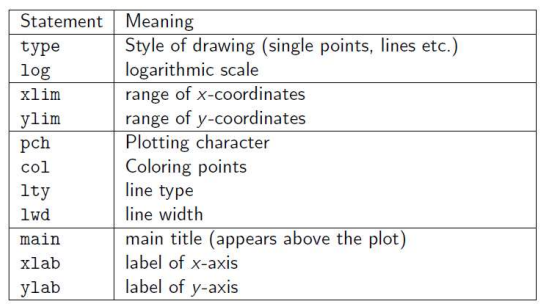
\includegraphics[keepaspectratio]{Plot_args.png}}
\caption{\textbf{Plot Arguments}}
\end{figure}

\textbf{Three categories of R graphics functions:}

• High-level plotting functions such as plot() to generate a new
graphics display.

• Low-level plotting functions such as legend() to add further graphical
elements to an existing plot.

• Interactive functions such as identify() to amend or collect
information interactively from a plot.

\textbf{Low-level plotting functions}

\begin{figure}
\centering
\pandocbounded{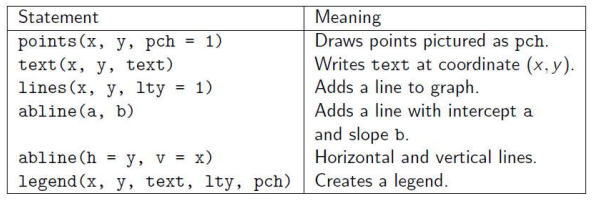
\includegraphics[keepaspectratio]{Low_level.png}}
\caption{Low-level plotting functions}
\end{figure}

\textbf{Useful plot functions}

\begin{itemize}
\tightlist
\item
  plot, pairs, interaction.plot
\item
  boxplot, hist
\item
  plot3d
\end{itemize}

\subsubsection{Graphical Output}\label{graphical-output}

\begin{Shaded}
\begin{Highlighting}[]
\FunctionTok{pdf}\NormalTok{(}\AttributeTok{file =} \StringTok{"iris\_plot.pdf"}\NormalTok{) }\CommentTok{\# open the graphics device}
\FunctionTok{plot}\NormalTok{(Sepal.Length }\SpecialCharTok{\textasciitilde{}}\NormalTok{ Sepal.Width, }\AttributeTok{data =}\NormalTok{ iris)}
\CommentTok{\# add anything else you want in your plots}
\FunctionTok{dev.off}\NormalTok{() }\CommentTok{\#close the graphic device}
\end{Highlighting}
\end{Shaded}

\begin{verbatim}
## pdf 
##   2
\end{verbatim}

Several plots in one graphical window: splits the graphical window into
3 rows and 2 columns.

\begin{Shaded}
\begin{Highlighting}[]
\FunctionTok{par}\NormalTok{(}\AttributeTok{mfrow=}\FunctionTok{c}\NormalTok{(}\DecValTok{3}\NormalTok{,}\DecValTok{2}\NormalTok{))}
\end{Highlighting}
\end{Shaded}

\textbf{Other Graphics: in lattice}

The lattice package functions: good for repeating graphs for various
groups. See the
\href{http://www.statmethods.net/advgraphs/trellis.html}{\textbf{Lattice
Graphs in R}} (at
\url{http://www.statmethods.net/advgraphs/trellis.html}) for more
information.

\begin{Shaded}
\begin{Highlighting}[]
\NormalTok{pacman}\SpecialCharTok{::}\FunctionTok{p\_load}\NormalTok{(lattice)}
\FunctionTok{xyplot}\NormalTok{(Sepal.Width }\SpecialCharTok{\textasciitilde{}}\NormalTok{ Sepal.Length }\SpecialCharTok{|}\NormalTok{ Species, }\AttributeTok{data =}\NormalTok{ iris)}
\end{Highlighting}
\end{Shaded}

\pandocbounded{\includegraphics[keepaspectratio]{SHC-798-R-code_files/figure-latex/lattice-1.pdf}}

\textbf{Other Graphics: in ggplot2}

\href{https://ggplot2.org}{\textbf{ggplot2}} package: very flexible,
based on grammar of graphics.

\begin{Shaded}
\begin{Highlighting}[]
\NormalTok{pacman}\SpecialCharTok{::}\FunctionTok{p\_load}\NormalTok{(ggplot2)}
\FunctionTok{ggplot}\NormalTok{(}\AttributeTok{data =}\NormalTok{ iris, }\FunctionTok{aes}\NormalTok{(}\AttributeTok{x =}\NormalTok{ Sepal.Length, }\AttributeTok{y =}\NormalTok{ Sepal.Width)) }\SpecialCharTok{+} \FunctionTok{facet\_grid}\NormalTok{(}\AttributeTok{rows =} \SpecialCharTok{\textasciitilde{}}\NormalTok{ Species) }\SpecialCharTok{+} \FunctionTok{geom\_point}\NormalTok{()}
\end{Highlighting}
\end{Shaded}

\pandocbounded{\includegraphics[keepaspectratio]{SHC-798-R-code_files/figure-latex/ggplot2-1.pdf}}

\subsection{Hypothesis Testing}\label{hypothesis-testing}

Approach: Hypothesis testing in 6 steps:

\begin{enumerate}
\def\labelenumi{\arabic{enumi}.}
\tightlist
\item
  Declare \emph{model} by which data were generated (e.g.~population is
  normally distributed, large sample size and σ not known).
\item
  Define null hypothesis, \textbf{H\textsubscript{0}} and alternative
  hypothesis, \textbf{H\textsubscript{A}} ; where
  \textbf{H\textsubscript{0}} is the statement being tested in a test of
  (statistical) significance and \textbf{H\textsubscript{A}} is the
  statement that is hoped or expected to be true instead of the null
  hypothesis
\item
  Choose the \emph{level of significance}, α.
\item
  Determine \emph{critical values} for the *level of significance α and
  \emph{degrees of freedom}, df = (n-1)
\item
  Define and calculate \textbf{test statistic}, e.g.~one-sample test:
\item
  \textbf{Compare} the test statistic to the \textbf{critical values}
  and make \textbf{decision} to \textbf{reject} or \textbf{fail to
  reject} H\textsubscript{0} .
\end{enumerate}

Hypothesis Tests -- An Example

\begin{Shaded}
\begin{Highlighting}[]
\CommentTok{\# Is the sepal length of versicolor different to that of virginica? Let’s use a *t{-}Test and a *Wilcoxon rank{-}sum test.}
\NormalTok{testdata }\OtherTok{\textless{}{-}}\NormalTok{ iris[iris}\SpecialCharTok{$}\NormalTok{Species }\SpecialCharTok{!=} \StringTok{"setosa"}\NormalTok{, }\FunctionTok{c}\NormalTok{(}\StringTok{"Sepal.Length"}\NormalTok{, }\StringTok{"Species"}\NormalTok{)]}
\NormalTok{testdata}\SpecialCharTok{$}\NormalTok{Species }\OtherTok{\textless{}{-}} \FunctionTok{droplevels}\NormalTok{(testdata}\SpecialCharTok{$}\NormalTok{Species)}
\FunctionTok{str}\NormalTok{(testdata) }\CommentTok{\# prepare and check the data}
\end{Highlighting}
\end{Shaded}

\begin{verbatim}
## 'data.frame':    100 obs. of  2 variables:
##  $ Sepal.Length: num  7 6.4 6.9 5.5 6.5 5.7 6.3 4.9 6.6 5.2 ...
##  $ Species     : Factor w/ 2 levels "versicolor","virginica": 1 1 1 1 1 1 1 1 1 1 ...
\end{verbatim}

\begin{Shaded}
\begin{Highlighting}[]
\CommentTok{\# Check normality assumption of t{-}Test using QQ{-}Plot:}
\NormalTok{versi.id }\OtherTok{\textless{}{-}}\NormalTok{ testdata}\SpecialCharTok{$}\NormalTok{Species }\SpecialCharTok{==} \StringTok{"versicolor"}
\FunctionTok{par}\NormalTok{(}\AttributeTok{mfrow=}\FunctionTok{c}\NormalTok{(}\DecValTok{1}\NormalTok{,}\DecValTok{2}\NormalTok{))}
\FunctionTok{qqnorm}\NormalTok{(testdata}\SpecialCharTok{$}\NormalTok{Sepal.Length[versi.id]); }\FunctionTok{qqline}\NormalTok{(testdata}\SpecialCharTok{$}\NormalTok{Sepal.Length[versi.id])}
\FunctionTok{qqnorm}\NormalTok{(testdata}\SpecialCharTok{$}\NormalTok{Sepal.Length[}\SpecialCharTok{!}\NormalTok{versi.id]); }\FunctionTok{qqline}\NormalTok{(testdata}\SpecialCharTok{$}\NormalTok{Sepal.Length[versi.id])}
\end{Highlighting}
\end{Shaded}

\pandocbounded{\includegraphics[keepaspectratio]{SHC-798-R-code_files/figure-latex/HT-1-sample-1.pdf}}

\begin{Shaded}
\begin{Highlighting}[]
\CommentTok{\# Two{-}sample t{-}test:}
\NormalTok{versi.id }\OtherTok{\textless{}{-}}\NormalTok{ testdata}\SpecialCharTok{$}\NormalTok{Species }\SpecialCharTok{==} \StringTok{"versicolor"}
\FunctionTok{t.test}\NormalTok{(}\AttributeTok{x =}\NormalTok{testdata}\SpecialCharTok{$}\NormalTok{Sepal.Length[versi.id], }\AttributeTok{y =}\NormalTok{ testdata}\SpecialCharTok{$}\NormalTok{Sepal.Length[}\SpecialCharTok{!}\NormalTok{versi.id], }\AttributeTok{var.equal =} \ConstantTok{TRUE}\NormalTok{)}
\end{Highlighting}
\end{Shaded}

\begin{verbatim}
## 
##  Two Sample t-test
## 
## data:  testdata$Sepal.Length[versi.id] and testdata$Sepal.Length[!versi.id]
## t = -5.6292, df = 98, p-value = 1.725e-07
## alternative hypothesis: true difference in means is not equal to 0
## 95 percent confidence interval:
##  -0.8818516 -0.4221484
## sample estimates:
## mean of x mean of y 
##     5.936     6.588
\end{verbatim}

\begin{Shaded}
\begin{Highlighting}[]
\CommentTok{\# T{-}test rejects the null hypothesis at 5\% significance level. Do not forget to visually check the normality assumptions (QQ{-}plot)}
\end{Highlighting}
\end{Shaded}

\begin{Shaded}
\begin{Highlighting}[]
\CommentTok{\# Check assumption of \textbackslash{}*Wilcoxon Rank Test: same distribution, just a location shift.}
\FunctionTok{boxplot}\NormalTok{(testdata}\SpecialCharTok{$}\NormalTok{Sepal.Length }\SpecialCharTok{\textasciitilde{}}\NormalTok{ testdata}\SpecialCharTok{$}\NormalTok{Species)}
\end{Highlighting}
\end{Shaded}

\pandocbounded{\includegraphics[keepaspectratio]{SHC-798-R-code_files/figure-latex/Wilcoxon-1.pdf}}

\begin{Shaded}
\begin{Highlighting}[]
\CommentTok{\# Now, perform the test:}
\NormalTok{versi.id }\OtherTok{\textless{}{-}}\NormalTok{ testdata}\SpecialCharTok{$}\NormalTok{Species }\SpecialCharTok{==} \StringTok{"versicolor"}
\FunctionTok{wilcox.test}\NormalTok{(}\AttributeTok{x =}\NormalTok{testdata}\SpecialCharTok{$}\NormalTok{Sepal.Length[versi.id], }\AttributeTok{y =}\NormalTok{ testdata}\SpecialCharTok{$}\NormalTok{Sepal.Length[}\SpecialCharTok{!}\NormalTok{versi.id], }\AttributeTok{var.equal =} \ConstantTok{TRUE}\NormalTok{)}
\end{Highlighting}
\end{Shaded}

\begin{verbatim}
## 
##  Wilcoxon rank sum test with continuity correction
## 
## data:  testdata$Sepal.Length[versi.id] and testdata$Sepal.Length[!versi.id]
## W = 526, p-value = 5.869e-07
## alternative hypothesis: true location shift is not equal to 0
\end{verbatim}

\begin{Shaded}
\begin{Highlighting}[]
\CommentTok{\# Wilcoxon Rank Test also rejects the null hypothesis at 5\% significance level. }
\end{Highlighting}
\end{Shaded}

The \textbf{Wilcoxon Rank Test} is the \emph{preferred} test for a
two-sample statistical test.

\subsubsection{Hypothesis Tests -
Summary}\label{hypothesis-tests---summary}

How to proceed:

\begin{itemize}
\tightlist
\item
  Formulate the null \& alternative hypotheses
\item
  Choose the appropriate test
\item
  Collate data, i.e., do an experiment
\item
  Look at data: plot(), pairs(), hist(), boxplot()
\item
  Validate assumptions of test (e.g., T-test, Wilcoxon test)
\item
  Carry out the test and interpret result
\end{itemize}

\begin{figure}
\centering
\pandocbounded{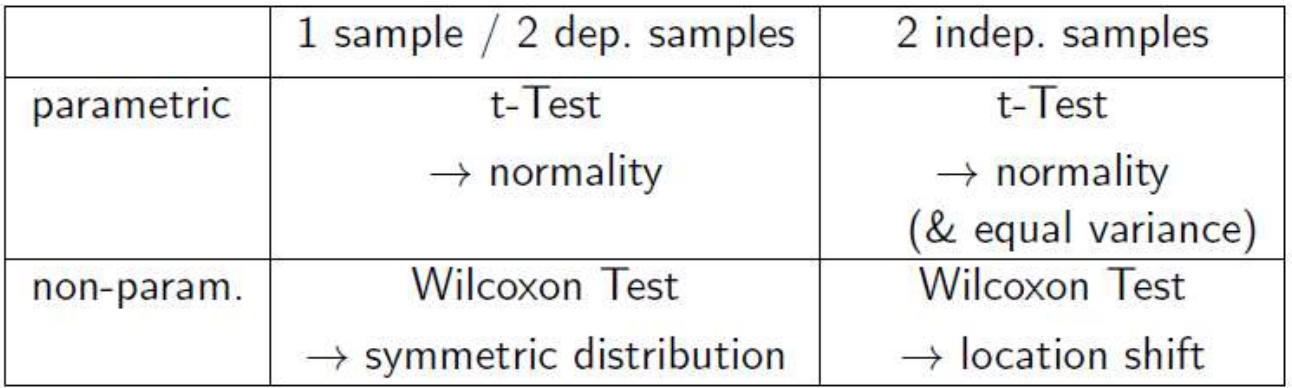
\includegraphics[keepaspectratio]{Hypothesis_Tests.png}}
\caption{Hypothesis Tests}
\end{figure}

Hypothesis Tests -- \textbf{Chi-squared test of independence}

\begin{itemize}
\tightlist
\item
  Hypothesis: H\textsubscript{0}: Independence of education and marriage
  status
\item
  H\textsubscript{A}: Dependence of education and marriage status
\end{itemize}

\begin{Shaded}
\begin{Highlighting}[]
\NormalTok{url }\OtherTok{\textless{}{-}} \StringTok{"https://stat.ethz.ch/Teaching/Datasets/edu.txt"}
\NormalTok{d.edu }\OtherTok{\textless{}{-}} \FunctionTok{read.table}\NormalTok{(url, }\AttributeTok{header =} \ConstantTok{TRUE}\NormalTok{)}

\CommentTok{\# Cross{-}tables in R}
\CommentTok{\# Count number of cases with same value:}
\FunctionTok{table}\NormalTok{(d.edu[, }\StringTok{"Married"}\NormalTok{])}
\end{Highlighting}
\end{Shaded}

\begin{verbatim}
## 
## Married more Married once 
##          205         1231
\end{verbatim}

\begin{Shaded}
\begin{Highlighting}[]
\CommentTok{\# Cross{-}table}
\FunctionTok{table}\NormalTok{(d.edu[, }\StringTok{"Education"}\NormalTok{], d.edu[, }\StringTok{"Married"}\NormalTok{])}
\end{Highlighting}
\end{Shaded}

\begin{verbatim}
##             
##              Married more Married once
##   College              61          550
##   No College          144          681
\end{verbatim}

\begin{Shaded}
\begin{Highlighting}[]
\CommentTok{\# Now we perform a Chi{-}squared test}
\FunctionTok{chisq.test}\NormalTok{(d.edu[, }\StringTok{"Education"}\NormalTok{], d.edu[, }\StringTok{"Married"}\NormalTok{])}
\end{Highlighting}
\end{Shaded}

\begin{verbatim}
## 
##  Pearson's Chi-squared test with Yates' continuity correction
## 
## data:  d.edu[, "Education"] and d.edu[, "Married"]
## X-squared = 15.405, df = 1, p-value = 8.675e-05
\end{verbatim}

\begin{Shaded}
\begin{Highlighting}[]
\CommentTok{\# Result: Reject H0, i.e. education and marriage are dependent.}
\end{Highlighting}
\end{Shaded}

\subsection{Correlation}\label{correlation}

\begin{Shaded}
\begin{Highlighting}[]
\CommentTok{\# Correlation}
\NormalTok{url1 }\OtherTok{\textless{}{-}} \StringTok{"https://stat.ethz.ch/Teaching/Datasets/basischOhneNA.dat"}
\NormalTok{d.basisch }\OtherTok{\textless{}{-}} \FunctionTok{read.table}\NormalTok{(url1, }\AttributeTok{header =} \ConstantTok{TRUE}\NormalTok{)}
\FunctionTok{str}\NormalTok{(d.basisch)}
\end{Highlighting}
\end{Shaded}

\begin{verbatim}
## 'data.frame':    123 obs. of  4 variables:
##  $ ph    : num  7.33 7.69 7.9 8.14 7.62 ...
##  $ l.sar : num  0.0969 0.4393 1 1.316 0.0607 ...
##  $ height: num  5.91 5.2 4.4 4.5 6.05 6 5.35 5.55 4.95 5.2 ...
##  $ h.quad: num  34.9 27 19.4 20.2 36.6 ...
\end{verbatim}

\begin{Shaded}
\begin{Highlighting}[]
\CommentTok{\# Calculate the (Pearson) correlation of ph and height:}
\FunctionTok{cor}\NormalTok{(d.basisch}\SpecialCharTok{$}\NormalTok{ph, d.basisch}\SpecialCharTok{$}\NormalTok{height)}
\end{Highlighting}
\end{Shaded}

\begin{verbatim}
## [1] -0.6925717
\end{verbatim}

\begin{Shaded}
\begin{Highlighting}[]
\CommentTok{\# Corresponding plot:}
\FunctionTok{plot}\NormalTok{(d.basisch}\SpecialCharTok{$}\NormalTok{ph, d.basisch}\SpecialCharTok{$}\NormalTok{height)}
\end{Highlighting}
\end{Shaded}

\pandocbounded{\includegraphics[keepaspectratio]{SHC-798-R-code_files/figure-latex/Correlation-1.pdf}}

All plots show 2 variables with a correlation of 0.7

\begin{itemize}
\tightlist
\item
  one looks good
\item
  another does not
\item
  outlier(s) influence the result
\item
  ALWAYS FIRST LOOK AT PLOTS
\end{itemize}

\subsection{Regression}\label{regression}

\subsubsection{Simple Linear Regression
(SLR)}\label{simple-linear-regression-slr}

From the d.basisch() data,

\begin{enumerate}
\def\labelenumi{\arabic{enumi}.}
\tightlist
\item
  \textbf{Response variable}: \emph{height} or h.quad: Height of trees
  or squared height, respectively.
\item
  \textbf{Possible explanatory variables}: \emph{ph}: pH-values of soil
  and l.sar: log(sodium absorption ratio)
\end{enumerate}

\begin{figure}
\centering
\pandocbounded{\includegraphics[keepaspectratio]{SLR-1.png}}
\caption{The Simple Linear Regression Model}
\end{figure}

Let us pick the variable ph as the explanatory variable.

\begin{Shaded}
\begin{Highlighting}[]
\CommentTok{\# Fit to data using lm:}
\NormalTok{fit }\OtherTok{\textless{}{-}} \FunctionTok{lm}\NormalTok{(}\AttributeTok{formula =}\NormalTok{ height }\SpecialCharTok{\textasciitilde{}}\NormalTok{ ph, }\AttributeTok{data =}\NormalTok{ d.basisch)}
\FunctionTok{summary}\NormalTok{(fit)}
\end{Highlighting}
\end{Shaded}

\begin{verbatim}
## 
## Call:
## lm(formula = height ~ ph, data = d.basisch)
## 
## Residuals:
##     Min      1Q  Median      3Q     Max 
## -3.7020 -0.5471  0.0874  0.6663  2.0033 
## 
## Coefficients:
##             Estimate Std. Error t value Pr(>|t|)    
## (Intercept)  28.7227     2.2395   12.82   <2e-16 ***
## ph           -3.0034     0.2844  -10.56   <2e-16 ***
## ---
## Signif. codes:  0 '***' 0.001 '**' 0.01 '*' 0.05 '.' 0.1 ' ' 1
## 
## Residual standard error: 1.008 on 121 degrees of freedom
## Multiple R-squared:  0.4797, Adjusted R-squared:  0.4754 
## F-statistic: 111.5 on 1 and 121 DF,  p-value: < 2.2e-16
\end{verbatim}

\begin{Shaded}
\begin{Highlighting}[]
\CommentTok{\# Estimated equation: height = 28.7 – 3.0pH}

\CommentTok{\# Drawing line into scatterplot:}
\FunctionTok{plot}\NormalTok{(d.basisch}\SpecialCharTok{$}\NormalTok{ph, d.basisch}\SpecialCharTok{$}\NormalTok{height) }\SpecialCharTok{+} \FunctionTok{abline}\NormalTok{(fit)}
\end{Highlighting}
\end{Shaded}

\pandocbounded{\includegraphics[keepaspectratio]{SHC-798-R-code_files/figure-latex/SLR-1.pdf}}

\begin{verbatim}
## integer(0)
\end{verbatim}

\begin{Shaded}
\begin{Highlighting}[]
\CommentTok{\# Fit to data using lm:}
\NormalTok{fit }\OtherTok{\textless{}{-}} \FunctionTok{lm}\NormalTok{(}\AttributeTok{formula =}\NormalTok{ height }\SpecialCharTok{\textasciitilde{}}\NormalTok{ ph, }\AttributeTok{data =}\NormalTok{ d.basisch)}
\FunctionTok{summary}\NormalTok{(fit)}
\end{Highlighting}
\end{Shaded}

\begin{verbatim}
## 
## Call:
## lm(formula = height ~ ph, data = d.basisch)
## 
## Residuals:
##     Min      1Q  Median      3Q     Max 
## -3.7020 -0.5471  0.0874  0.6663  2.0033 
## 
## Coefficients:
##             Estimate Std. Error t value Pr(>|t|)    
## (Intercept)  28.7227     2.2395   12.82   <2e-16 ***
## ph           -3.0034     0.2844  -10.56   <2e-16 ***
## ---
## Signif. codes:  0 '***' 0.001 '**' 0.01 '*' 0.05 '.' 0.1 ' ' 1
## 
## Residual standard error: 1.008 on 121 degrees of freedom
## Multiple R-squared:  0.4797, Adjusted R-squared:  0.4754 
## F-statistic: 111.5 on 1 and 121 DF,  p-value: < 2.2e-16
\end{verbatim}

\begin{Shaded}
\begin{Highlighting}[]
\CommentTok{\# Estimated equation: height = 28.7 – 3.0pH}

\CommentTok{\# Drawing line into scatterplot:}
\FunctionTok{plot}\NormalTok{(d.basisch}\SpecialCharTok{$}\NormalTok{ph, d.basisch}\SpecialCharTok{$}\NormalTok{height) }\SpecialCharTok{+} \FunctionTok{abline}\NormalTok{(fit)}
\end{Highlighting}
\end{Shaded}

\begin{verbatim}
## integer(0)
\end{verbatim}

\paragraph{SLR - Residual Analysis}\label{slr---residual-analysis}

Diagnostics plots are straightforward:

\begin{Shaded}
\begin{Highlighting}[]
\FunctionTok{par}\NormalTok{(}\AttributeTok{mfrow =} \FunctionTok{c}\NormalTok{(}\DecValTok{2}\NormalTok{,}\DecValTok{2}\NormalTok{))}
\FunctionTok{plot}\NormalTok{(fit)}
\end{Highlighting}
\end{Shaded}

\pandocbounded{\includegraphics[keepaspectratio]{SHC-798-R-code_files/figure-latex/SLR-Resid1-1.pdf}}

\begin{enumerate}
\def\labelenumi{\arabic{enumi}.}
\tightlist
\item
  Tukey-Anscombe plot (is the variance of the errors Ei constant? Is the
  regression function correct?)
\item
  Q-Q plot (are the errors Ei normally distributed?)
\item
  Scale location plot (similar to Tukey-Anscombe plot)
\item
  Leverage plot (what points have a strong influence on the fit?)
\end{enumerate}

Residual plots by hand:

\begin{Shaded}
\begin{Highlighting}[]
\FunctionTok{par}\NormalTok{(}\AttributeTok{mfrow =} \FunctionTok{c}\NormalTok{(}\DecValTok{1}\NormalTok{,}\DecValTok{2}\NormalTok{))}
\FunctionTok{plot}\NormalTok{(fit}\SpecialCharTok{$}\NormalTok{fitted,fit}\SpecialCharTok{$}\NormalTok{resid) }

\CommentTok{\#Tukey{-}Anscombe}
\FunctionTok{qqnorm}\NormalTok{(fit}\SpecialCharTok{$}\NormalTok{resid) }\CommentTok{\#quantil{-}Quantil Plot}
\FunctionTok{qqline}\NormalTok{(fit}\SpecialCharTok{$}\NormalTok{resid) }\CommentTok{\# adds the diagonal line}
\end{Highlighting}
\end{Shaded}

\pandocbounded{\includegraphics[keepaspectratio]{SHC-798-R-code_files/figure-latex/SLR-Resid2-1.pdf}}

\begin{figure}
\centering
\pandocbounded{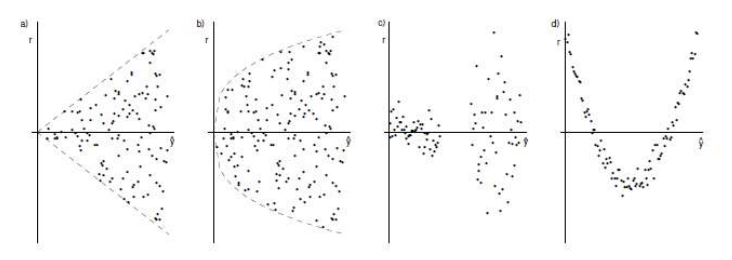
\includegraphics[keepaspectratio]{Bad-TA-Plots.png}}
\caption{Some bad Tukey-Anscombe plots}
\end{figure}

\subsubsection{Multiple Linear
Regression}\label{multiple-linear-regression}

Expand the simple linear model to more than one explanatory variable.

\begin{figure}
\centering
\pandocbounded{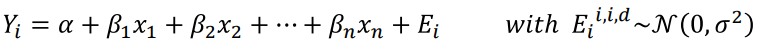
\includegraphics[keepaspectratio]{MLR.png}}
\caption{The Multiple Linear Regression Model}
\end{figure}

\begin{Shaded}
\begin{Highlighting}[]
\CommentTok{\# Fit the model with lm}
\NormalTok{fitm }\OtherTok{\textless{}{-}} \FunctionTok{lm}\NormalTok{(height }\SpecialCharTok{\textasciitilde{}}\NormalTok{ ph }\SpecialCharTok{+}\NormalTok{ l.sar, }\AttributeTok{data =}\NormalTok{ d.basisch)}
\FunctionTok{summary}\NormalTok{(fitm)}
\end{Highlighting}
\end{Shaded}

\begin{verbatim}
## 
## Call:
## lm(formula = height ~ ph + l.sar, data = d.basisch)
## 
## Residuals:
##     Min      1Q  Median      3Q     Max 
## -4.1314 -0.4911  0.0849  0.6488  2.4754 
## 
## Coefficients:
##             Estimate Std. Error t value Pr(>|t|)    
## (Intercept)  26.9466     2.7445   9.818  < 2e-16 ***
## ph           -2.7558     0.3603  -7.649  5.6e-12 ***
## l.sar        -0.2519     0.2255  -1.117    0.266    
## ---
## Signif. codes:  0 '***' 0.001 '**' 0.01 '*' 0.05 '.' 0.1 ' ' 1
## 
## Residual standard error: 1.007 on 120 degrees of freedom
## Multiple R-squared:  0.485,  Adjusted R-squared:  0.4764 
## F-statistic: 56.51 on 2 and 120 DF,  p-value: < 2.2e-16
\end{verbatim}

\paragraph{MLR - Residual Analysis}\label{mlr---residual-analysis}

\begin{Shaded}
\begin{Highlighting}[]
\CommentTok{\# Look at the same plots as for simple linear regression}
\FunctionTok{plot}\NormalTok{(fitm)}
\end{Highlighting}
\end{Shaded}

\pandocbounded{\includegraphics[keepaspectratio]{SHC-798-R-code_files/figure-latex/MLR-Resid-1.pdf}}
\pandocbounded{\includegraphics[keepaspectratio]{SHC-798-R-code_files/figure-latex/MLR-Resid-2.pdf}}
\pandocbounded{\includegraphics[keepaspectratio]{SHC-798-R-code_files/figure-latex/MLR-Resid-3.pdf}}
\pandocbounded{\includegraphics[keepaspectratio]{SHC-798-R-code_files/figure-latex/MLR-Resid-4.pdf}}

\begin{Shaded}
\begin{Highlighting}[]
\CommentTok{\# It may help to plot the explanatory variables against the residuals.}
\FunctionTok{plot}\NormalTok{(d.basisch}\SpecialCharTok{$}\NormalTok{ph, fitm}\SpecialCharTok{$}\NormalTok{resid)}
\end{Highlighting}
\end{Shaded}

\pandocbounded{\includegraphics[keepaspectratio]{SHC-798-R-code_files/figure-latex/MLR-Resid-5.pdf}}

\begin{Shaded}
\begin{Highlighting}[]
\FunctionTok{plot}\NormalTok{(d.basisch}\SpecialCharTok{$}\NormalTok{l.sar, fitm}\SpecialCharTok{$}\NormalTok{resid)}
\end{Highlighting}
\end{Shaded}

\pandocbounded{\includegraphics[keepaspectratio]{SHC-798-R-code_files/figure-latex/MLR-Resid-6.pdf}}

\end{document}
